%%%%%%%%%%%%%%%%%%%%%%%%%%%%%%%%%%%%%%%%%%%%%%%%%%%%%%%%%%%%%%%%%%%%%%%%%%%%%%%
% Chapter 2: Conceptos
%%%%%%%%%%%%%%%%%%%%%%%%%%%%%%%%%%%%%%%%%%%%%%%%%%%%%%%%%%%%%%%%%%%%%%%%%%%%%%%

%++++++++++++++++++++++++++++++++++++++++++++++++++++++++++++++++++++++++++++++
En este capítulo se abordarán todos aquellos conceptos teóricos que han surgido
a lo largo del proyecto y son necesarios para entender correctamente la línea
del trabajo.


%++++++++++++++++++++++++++++++++++++++++++++++++++++++++++++++++++++++++++++++
\section{Visión artificial}
\label{2:sec:1}
%%%%%%%%%%%%%%%%%%%%%%%%%%%%%%%%%%%%%%%%%%%%%%%%%%%%%%%%%%%%%%%%%%%%%%%%%%%%%%%%
% Chapter 2: Conceptos
%%%%%%%%%%%%%%%%%%%%%%%%%%%%%%%%%%%%%%%%%%%%%%%%%%%%%%%%%%%%%%%%%%%%%%%%%%%%%%%%

%++++++++++++++++++++++++++++++++++++++++++++++++++++++++++++++++++++++++++++++
% \section{Visión artificial}
% \label{2:sec:1}
% https://campusvirtual.ull.es/1516/course/view.php?id=202
% https://es.wikipedia.org/wiki/Visi%C3%B3n_artificial
% https://en.wikipedia.org/wiki/Computer_vision
% J. GONZÁLEZ JIMÉNEZ, "Visión Por Computador", Editorial Paraninfo. 2000

La visión artificial por computador, es la disciplina científica que se basa en
la adquisición, procesamiento y análisis de las imágenes que se toman del mundo
real, con el objetivo de obtener información relevante acerca de ellas:
detección de objetos, seguimiento del movimiento, reconocimiento de eventos,
etc. Un ejemplo que podemos ver en nuestro día a día, es la detección de caras
en una escena capturada por una cámara digital o smartphone, mediante el uso de
técnicas de reconocimiento de patrones.

Al igual que sucede en otras áreas de la inteligencia artificial, la visión
artificial tiene como objetivo principal obtener la información explícita y el
significado de la realidad de la misma manera que lo haría un ser biológico.

El avance progresivo del hardware con nuevos procesadores digitales de señales
(DSP) y unidades de procesamiento gráfico (GPU), junto con nuevas tecnologías y
planteamientos de cómputo como la computación paralela, ha permitido que en los
últimos años se haya podido implementar nuevos algoritmos más rápidos y
eficientes, necesarios para ser utilizados en ámbitos críticos, como sistemas
en tiempo real.

%+++++++++++++++++++++++++++++++++++++++++++++++++++++++++++++++++++++++++++++++
\subsection{Dificultades}
La capacidad visual es uno pilares de la inteligencia humana. Su implementación
en la rotótica supone también un importante avance en la inteligencia
artificial. Sin embargo, mientras que la percepción visual es algo innato y
cotidiano para nosotros, la visión artificial es muy compleja y conlleva muchas
dificultades. Entre las principales dificultades, destacan:

\begin{itemize}
  \item \textbf{Mundo tridimensional:} mientras que las imágenes que se
  obtienen con una cámara son bidimensionales, el mundo que nos rodea no. Es
  necesario realizar las transformaciones correspondientes para obtener valores
  correctos.
  \item \textbf{Zonas de interés:} se necesita extraer elementos de información 
  sutiles en imágenes complejas, por lo que entre tanta información es
  necesario reconocer formas, colores, etc.
  \item \textbf{Carácter dinámico de las escenas:} el mundo está vivo, por lo
  que en las imágenes que se toman muchos elementos están en movimiento. Por 
  otro lado, otros factores como luminosidad, contraste, foco... pueden marcar
  una importante diferencia, y por desgracia, estos factores son variables, no
  se pueden controlar.
\end{itemize}

%+++++++++++++++++++++++++++++++++++++++++++++++++++++++++++++++++++++++++++++++
\subsection{Aplicaciones}
% https://www.ptgrey.com/tan/10570
La visión artificial resulta de gran utilidad en diferentes áreas de
aplicación, tanto en acciones repetitivas como peligrosas:


\begin{itemize}
  \item \textbf{Inspección y ensamblaje industrial:} el proyecto "Randon Bin
  Picking" (RBP) hace uso de visión estéreo para la búsqueda de piezas entre
  objetos de todo tipo para su rápida recuperación.
  % http://www.worldscientific.com/doi/suppl/10.1142/8766/suppl_file/8766_chap01.pdf
  \item \textbf{Apoyo en el diagnóstico médico:} en las últimas décadas la
  visión artificial se ha hecho un importante en la medicina para detectar,
  analizar y reconstruir la información obtenida.
  % http://www.ri.cmu.edu/pub_files/pub4/matthies_larry_2007_1/matthies_larry_2007_1.pdf
  \item \textbf{Exploración espacial:} en el proyecto de exploración Mars Rover
  (Mars Exploration Rover Mission) tiene como objetivo explorar la superficie
  de Marte en busca de rocas u otros elementos que prueben la existencia de
  agua.
  \item \textbf{Seguimiento (Tracking):} se hace uso en innumerables
  situaciones de carácter estadístico como contar el número o de en áreas de
  vigilancia y seguridad monitorizando trayectorias.
\end{itemize}

%++++++++++++++++++++++++++++++++++++++++++++++++++++++++++++++++++++++++++++++


%++++++++++++++++++++++++++++++++++++++++++++++++++++++++++++++++++++++++++++++
\section{Visión estéreo}
\label{2:sec:2}
%%%%%%%%%%%%%%%%%%%%%%%%%%%%%%%%%%%%%%%%%%%%%%%%%%%%%%%%%%%%%%%%%%%%%%%%%%%%%%%%
% Chapter 2: Conceptos
%%%%%%%%%%%%%%%%%%%%%%%%%%%%%%%%%%%%%%%%%%%%%%%%%%%%%%%%%%%%%%%%%%%%%%%%%%%%%%%%

%++++++++++++++++++++++++++++++++++++++++++++++++++++++++++++++++++++++++++++++
% \section{Visión estéreo}
% \label{2:sec:2}

La visión estereoscópica o visión estéreo, es la técnica capaz de extraer
información tridimensional (profundidad) a partir de la posición relativa de un
objeto en imágenes bidimensionales al ser observado desde distintos ángulo por
dos o más cámaras separadas a una cierta distancia.

%+++++++++++++++++++++++++++++++++++++++++++++++++++++++++++++++++++++++++++++++
% \subsection{Calibración}

%+++++++++++++++++++++++++++++++++++++++++++++++++++++++++++++++++++++++++++++++
\subsection{Adquisición}

Usando dos cámaras, el procedimiento a seguir para la adquisición del entorno
es capturar dos imágenes de una misma escena, desde dos cámaras separadas
ligeramente. De esta forma, las imágenes obtenidas, también tendrán un pequeño 
desplazamiento entre sí.

De manera más formal, se obtiene que para cada imagen capturada por las
cámaras, un objeto está en puntos diferentes del plano. Esta triangulación
entre el punto P y Q y el origen de referencia, provocan una sensación de
profundidad. Mediante el sistema tradicional de una sola cámara, este punto
estaría en las mismas coordenadas \cite{VisionEstereo}.

\begin{figure}[!th]
  \begin{center}
    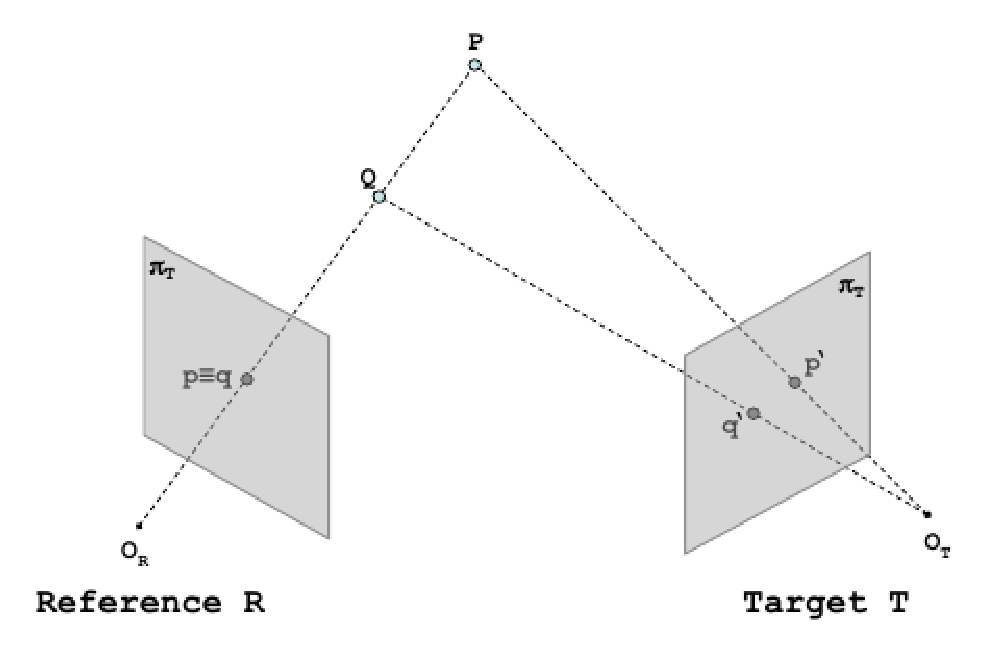
\includegraphics[width=0.5\textwidth]{images/cap2/VisionEstereo.eps}
    \caption{Diferencias entre una y dos cámaras}
    \label{fig:VisionEstereo}
  \end{center}
\end{figure}

Con estos datos, se pueden poner en correspondencia cada punto de ambas
imágenes, para obtener una imagen de disparidad (más información en la sección 
~\ref{subsec:Disparidad}).

%+++++++++++++++++++++++++++++++++++++++++++++++++++++++++++++++++++++++++++++++
\subsection{Geometría de las cámaras}
En función de la posición relativa de las cámaras entre sí, se pueden apreciar
dos métodos principales:

\begin{itemize}
  \item \textbf{Visión paralela:} las cámaras están paralelas entre sí y están
  separadas por una línea horizontal (línea base). El objetivo que visualiza
  cada cámara es perpendicular respecto a la línea base, mientras que las
  líneas de correspondencia que unen los puntos de una imagen respecto a la
  otra son horizontales.

  \begin{minipage}{\linewidth}
      \centering
      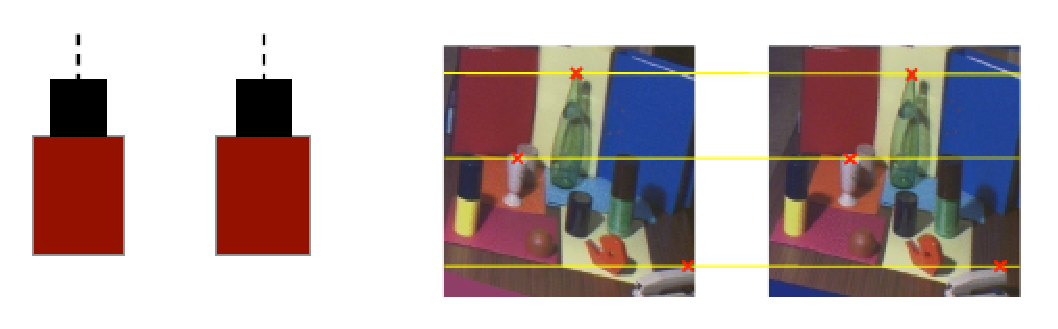
\includegraphics[width=0.6\textwidth]{images/cap2/VisionParalela.eps}
      \captionof{figure}{Visión paralela}
      \label{fig:VisionParalela}
  \end{minipage}

  \item \textbf{Visión cruzada:} las cámaras no están paralelas entre sí,
  tienen una inclinación de tal forma que el objetivo de cada cámara apunta
  hacia el lado contrario de una imagen. Por lo que los ejes ópticos se cruzan
  entre sí. Las líneas de correspondencia, también tienen sufren una
  inclinación.

  \begin{minipage}{\linewidth}
      \centering
      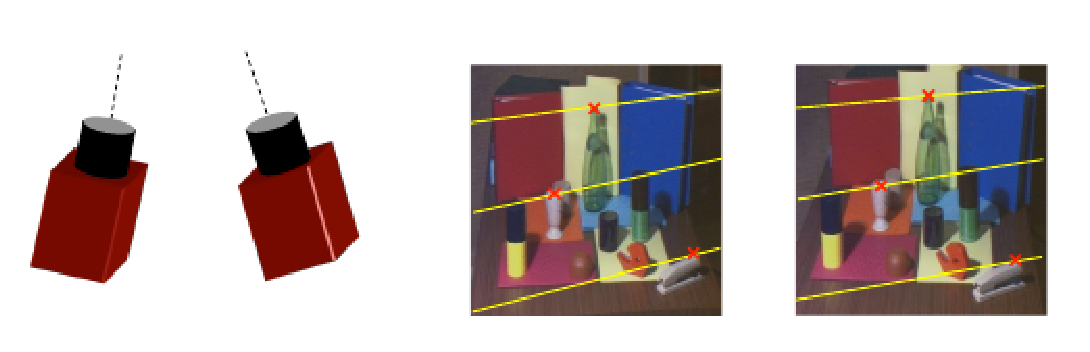
\includegraphics[width=0.6\textwidth]{images/cap2/VisionCruzada.eps}
      \captionof{figure}{Visión cruzada}
      \label{fig:VisionCruzada}
  \end{minipage}
\end{itemize}

La visión cruzada tiene la desventaja de distorsionar las imágenes capturadas.
En la figura ~\ref{fig:VisionCruzadaMuro} se puede observar este efecto al
fotografiar un muro de ladrillos. Sin embargo, dependiendo del tipo de escena
que se capture, esta distorsión puede suponer un problema o no \cite{Geometria}.

\begin{figure}[!th]
  \begin{center}
    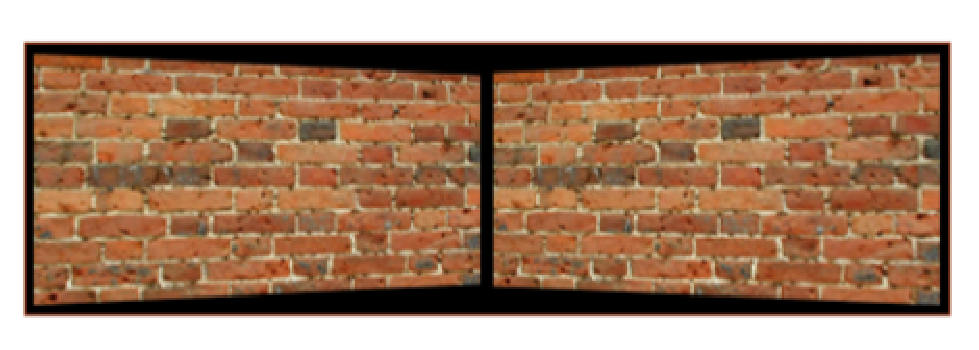
\includegraphics[width=0.5\textwidth]{images/cap2/VisionCruzadaMuro.eps}
    \caption{Muro distorsionado por visión cruzada}
    \label{fig:VisionCruzadaMuro}
  \end{center}
\end{figure}


% Ampliar o quitar
% La visión paralela por su parte, no distorsiona las imágenes capturadas, pero
% también cuenta con otra serie de problemas. A pesar de ello, la visión paralela
% suele ser la más utilizada para la visión estéreo.

%+++++++++++++++++++++++++++++++++++++++++++++++++++++++++++++++++++++++++++++++
% \subsection{Rectificación}
% https://en.wikipedia.org/wiki/Image_rectification

%+++++++++++++++++++++++++++++++++++++++++++++++++++++++++++++++++++++++++++++++
\subsection{Disparidad}
\label{subsec:Disparidad}
% http://es.slideshare.net/RicardoSnchezCastill/vision-artificial-49264591
% http://stackoverflow.com/questions/17607312/difference-between-disparity-map-and-disparity-image-in-stereo-matching

La disparidad de dos imágenes establece la correspondencia entre los píxeles o
características que existen entre ambas en el eje x para obtener la profundidad
de la escena. Con esto se consigue estimar la profundidad de cada uno de los
puntos en la escena.

El objetivo final es poder construir una \textbf{imagen o mapa de disparidad},
una imagen que representa la disparidad entre las dos cámaras. Habitualmente
el mapa de disparidad se representa como una imagen monocroma donde los objetos
con mayor disparidad (más cercanos) son representados con un tono más claro y
los objetos con menor disparidad (más lejanos) son representados con un tono más
oscuro. Aunque no es extraño encontrar una imagen térmica en vez de monocroma.

Con el único requisito de que las imágenes estén rectificadas, el algoritmo para
calcular la disparidad consiste de forma general en buscar cada punto singular
de la imagen izquierda en la imagen derecha, para observa en que nuevo píxel se
encuentra. A partir de esta información, es posible calcular la profundidad
buscando para cada punto de las imágenes la pareja de puntos correspondiente que
representan la proyección del mismo punto del espacio \cite{CalculoDisparidad}.

El mapa de disparidad es uno de los elementos básicos para la reconstrucción
tridimensional de los objetos de una escenas a partir de varias capturas.

\begin{figure}[!th]
  \begin{center}
    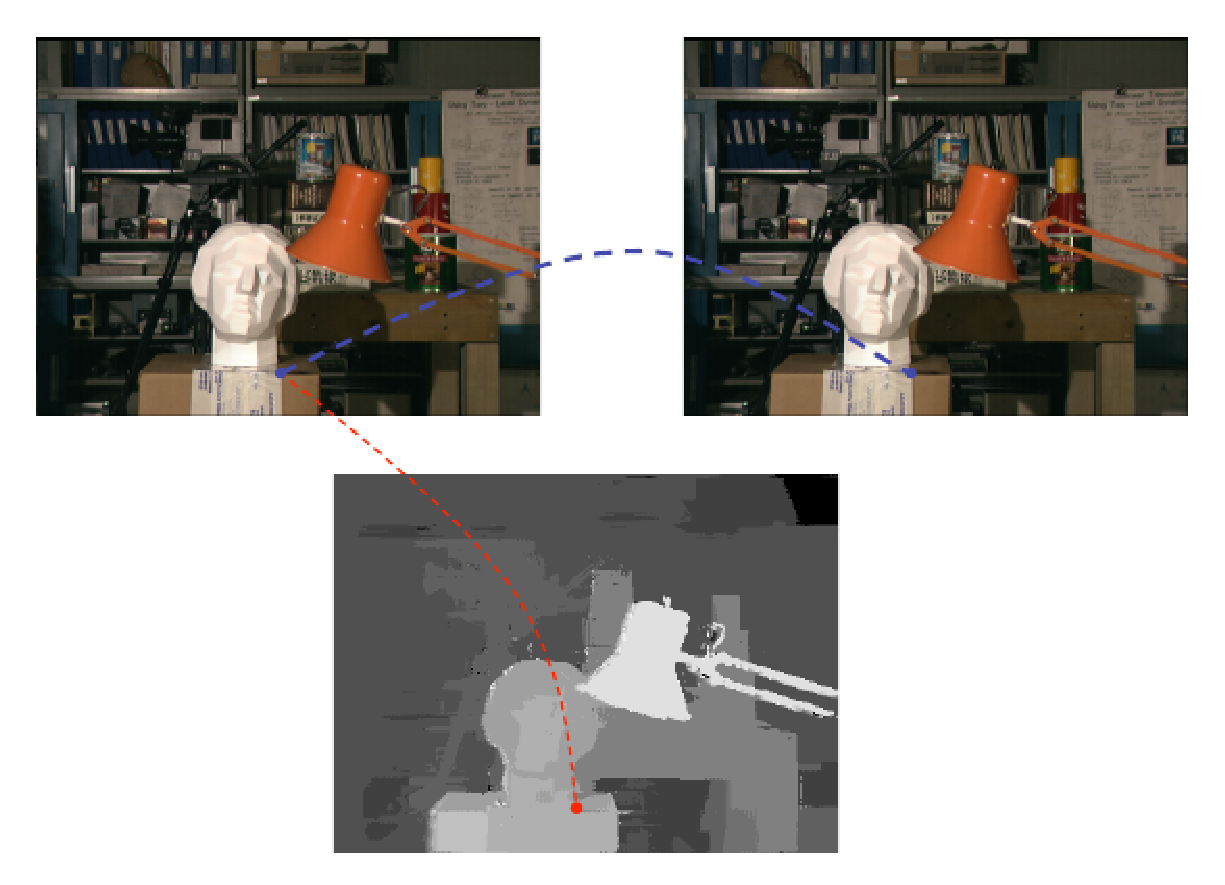
\includegraphics[width=0.6\textwidth]{images/cap2/MapaDisparidad.eps}
    \caption{Mapa de disparidad a partir de imágenes en estéreo}
    \label{fig:MapaDisparidad}
  \end{center}
\end{figure}

%+++++++++++++++++++++++++++++++++++++++++++++++++++++++++++++++++++++++++++++++
% \subsection{Reconstrucción 3D}

%++++++++++++++++++++++++++++++++++++++++++++++++++++++++++++++++++++++++++++++


%++++++++++++++++++++++++++++++++++++++++++++++++++++++++++++++++++++++++++++++
\section{Odometría}
\label{2:sec:3}
%%%%%%%%%%%%%%%%%%%%%%%%%%%%%%%%%%%%%%%%%%%%%%%%%%%%%%%%%%%%%%%%%%%%%%%%%%%%%%%%
% Chapter 2: Conceptos
%%%%%%%%%%%%%%%%%%%%%%%%%%%%%%%%%%%%%%%%%%%%%%%%%%%%%%%%%%%%%%%%%%%%%%%%%%%%%%%%

%++++++++++++++++++++++++++++++++++++++++++++++++++++++++++++++++++++++++++++++
% \section{Odometría}
% \label{2:sec:3}

La odometría es el método que permite estimar la posición de un robot móvil en
el entorno en un momento determinado. 

Cabe recalcar, que la odometría no permite conocer la posición exacta de un
robot, ya que existen muchos factores externos, que provocan errores en la
obtención de los datos de entrada. Estos errores son acumulativos, por lo que
la veracidad de los resultados es inversamente proporcional a la distancia
recorrida de un robot.

A pesar de ello, la odometría ofrece una gran precisión a corto plazo y su
precio de implementación es realmente bajo, por lo que lo convierte en uno de
los pilares básicos para la navegación. 

Dependiendo de la tecnología utilizada para cálcular la odometría, se puede 
hablar de diferentes tipos.

%+++++++++++++++++++++++++++++++++++++++++++++++++++++++++++++++++++++++++++++++
\subsection{Odometría mecánica}
% https://es.wikipedia.org/wiki/Odometr%C3%ADa
La odometría mecánica se base en el estudio del giro de las ruedas de un robot.
Conociendo el radio de las ruedas, mediante las revoluciones de las mismas es
posible determinar con sencillas ecuaciones el avance del robot.

Sin embargo esta sencilla solución tiene varios inconvenientes a tratar:

\begin{itemize}
  \item \textbf{Las ruedas:} las ruedas utilizadas deben contar con las mismas
  características, pero en muchas cosasiones el diámetro de las ruedas es
  diferente, o simplemente el diámetro no se corresponde con las
  especificaciones dadas por el fabricante. Por otro lado es necesario que las
  ruedas se encuentren bien alineadas.
  \item \textbf{El entorno:} la superficie por donde se mueve el robot puede no
  ser la adecuada. Dependiendo de la composición del suelo (gravilla, hierba,
  baldosas, etc), el robot puede resbalar, derrapar o incluso encontrarse sin
  ingún punto de contacto con el suelo. Por otra parte, una superficie
  desnivelada o llena de obstáculos inesperados también supone un problema para
  obtener la odometría.
\end{itemize}


%+++++++++++++++++++++++++++++++++++++++++++++++++++++++++++++++++++++++++++++++
\subsection{Odometría visual}
% https://prezi.com/tl9fmj3cs4ai/sistema-de-odometria-visual-estimacion-de-la-localizacion-d/
La odometría visual permite estimar el movimiento y la posición de un robot
móvil a partir de las imágenes capturadas por una o más cámaras en el propio
sistema. De forma sencilla, si se comparan las imágenes obtenidas en un instante
t1 respecto a otras imágenes obtenidas en un instante t2, se puede calcular la
diferencia existente en un punto determinado de la imagen. Si dicho punto está
más cerca, quiere decir que el robot ha avanzado.

Pero a partir de las imágenes ¿cómo se puede determinar la distancia de un
objeto respecto al robot? En función del tamaño del objeto en la escena. Si en
la nueva escena las dimensiones espaciales de un objeto son mayores que la
anterior escena, quiere decir que se ha avanzado, y viceversa. En un sistema
esterereoscópico se comparan la diferencia respecto al eje x (disparidad) entre
la imagen izquierda y derecha. La distancia de un objeto es inversamente
proporcional a la disparidad presente, es decir, si un objeto presenta una gran
disparidad en la escena significa que se encuentra cerca. Cuanto más lejano esté
el objeto la disparidad será menor.

% \begin{wrapfigure}{l}{0.5\textwidth}
%   \vspace{-20pt}
%   \begin{center}
%     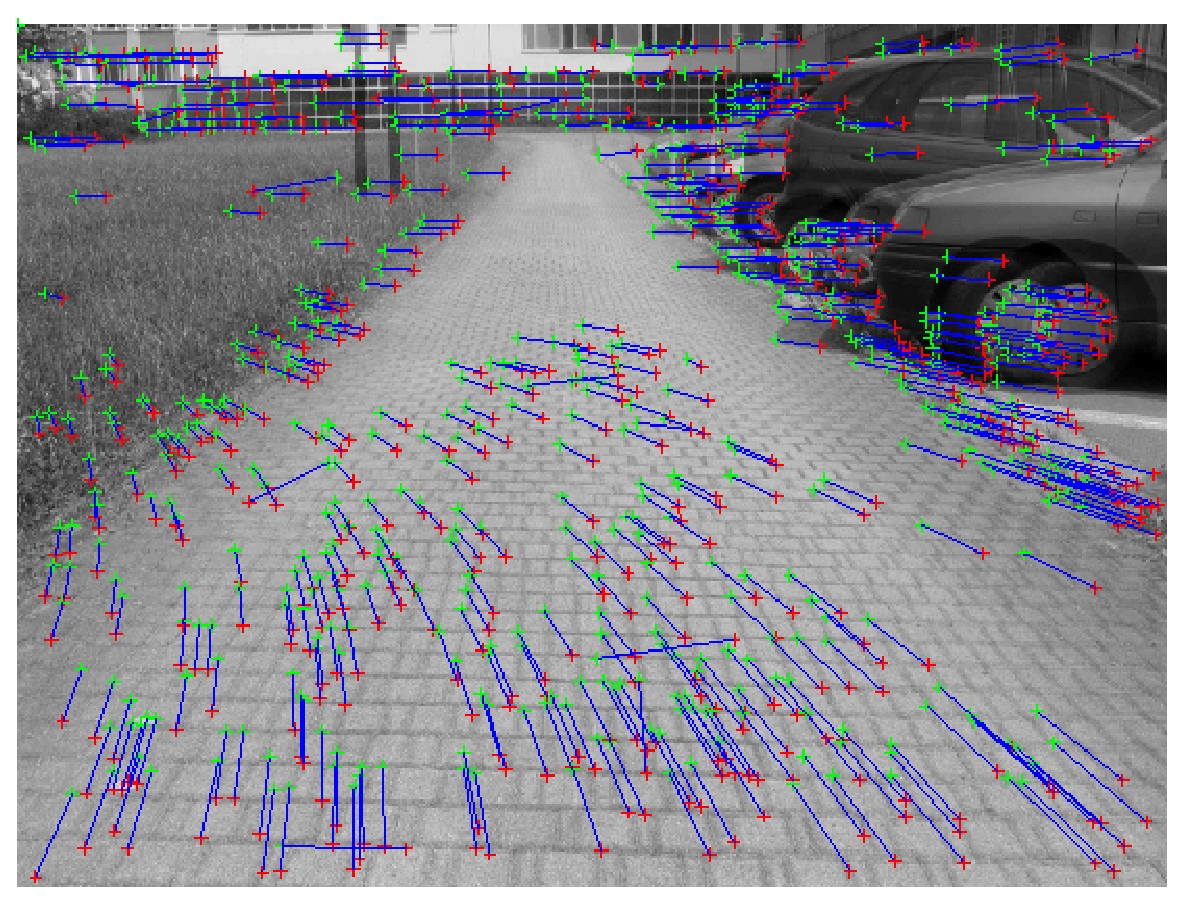
\includegraphics[width=0.48\textwidth]{images/cap2/OdometriaVisual.eps}
%   \end{center}
%   \vspace{-20pt}
%   \caption{Disparidad en odometría visual}
%   \vspace{-10pt}
%   \label{fig:OdometriaVisual}
% \end{wrapfigure}

\begin{minipage}{\linewidth}
    \centering
    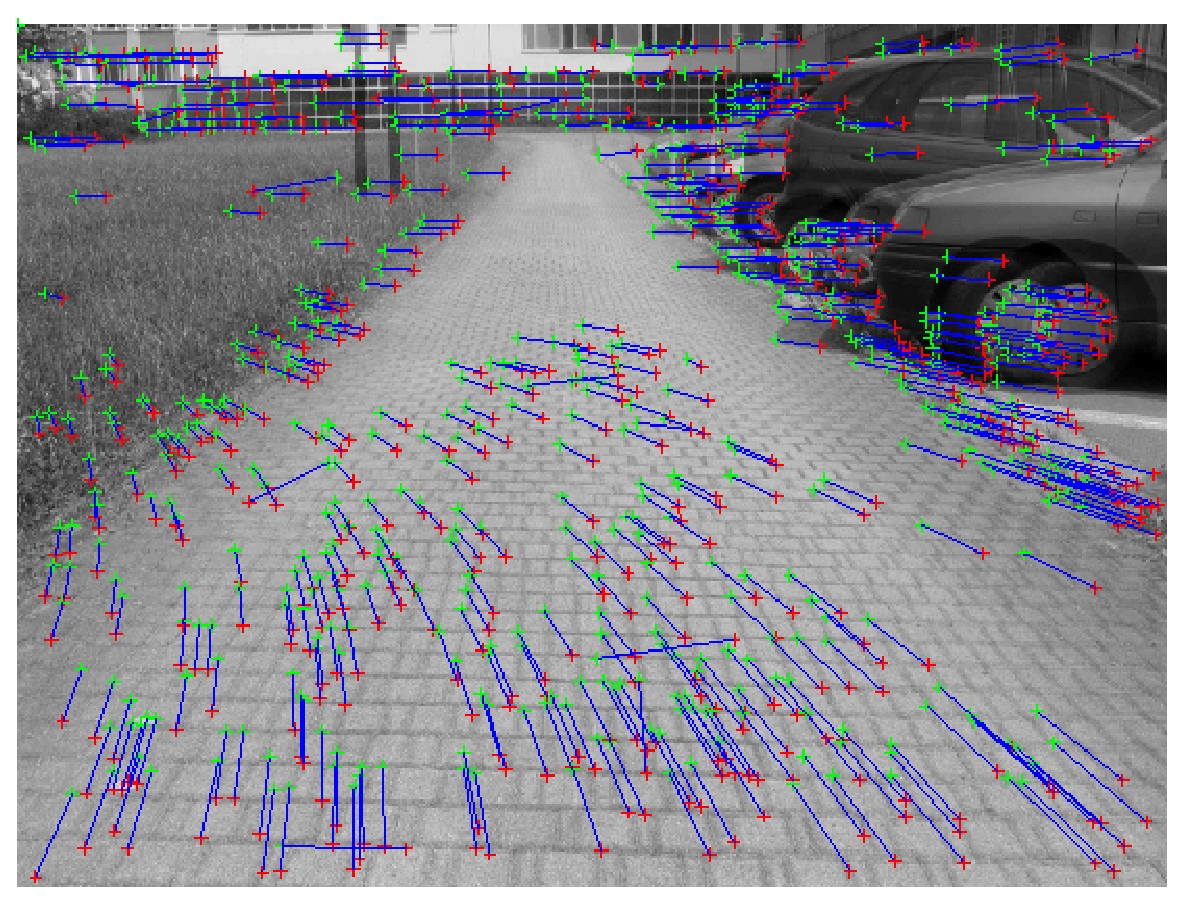
\includegraphics[width=0.5\textwidth]{images/cap2/OdometriaVisual.eps}
    \captionof{figure}{Disparidad en odometría visual}
    \label{fig:OdometriaVisual}
\end{minipage}

La odometría visual es la alternativa utilizada en robots móviles que no cuentan
con ruedas: androides, robots voladores, etc. Aunque también es bastante
frecuente encontrar la odometría visual junto con la odométría mecánica como
apoyo.

La odometría visual cuenta con los siguientes inconvenientes a tener en cuenta:

\begin{itemize}
  \item \textbf{Las cámaras:} para funcionar correctamente, es necesario que las
  cámaras estén calibradas. Por otra parte, si se utiliza un sistema
  estereóscopico se necesita verificar que la distancia entre las cámaras sea la
  correcta.
  \item \textbf{El entorno:} las cámaras son muy sencibles a los cambios bruscos
  de las condiciones del entorno como la luminosidad. También hay que tener en
  cuenta que las escenas son dinámicas, por lo que muchos objetos aparecen y
  desparecen dela escena o se mueven con mucha frecuencia en la escena, y esto
  puede suponer un importante problema.
\end{itemize}
    
Tanto la odometría mecánica como la visual presentan varios problemas para
estimar la posición y orientación del robot, sin embargo, combinando ambas se
pueden conseguir resultados más consistentes. Por ejemplo: en aquellos casos
donde la odometría mecánica no coincide con los datos visuales debido a una
superficie inconsistente, se confía en la odometría visual. Por otra parte,
cuando las condiciones lumínicas no son adecuadas, se confía en la odometría
mecánica.

%++++++++++++++++++++++++++++++++++++++++++++++++++++++++++++++++++++++++++++++


%++++++++++++++++++++++++++++++++++++++++++++++++++++++++++++++++++++++++++++++
\section{Navegación robótica}
\label{2:sec:4}
%%%%%%%%%%%%%%%%%%%%%%%%%%%%%%%%%%%%%%%%%%%%%%%%%%%%%%%%%%%%%%%%%%%%%%%%%%%%%%%%
% Chapter 2: Conceptos
%%%%%%%%%%%%%%%%%%%%%%%%%%%%%%%%%%%%%%%%%%%%%%%%%%%%%%%%%%%%%%%%%%%%%%%%%%%%%%%%

%++++++++++++++++++++++++++++++++++++++++++++++++++++++++++++++++++++++++++++++
% \section{Navegación robótica}
% \label{2:sec:4}
% https://en.wikipedia.org/wiki/Mobile_robot_navigation
La navegación robótica es la habilidad que permite a un robot móvil poder
localizarse en el entorno y poder moverse libremente por el mismo, a partir del
conocimiento extraído de las imágenes obtenidas del medio. El objetivo principal
es conocer por donde debe y no debe navegar con la idea de poder alcanzar un
punto de destino marcado previamente. 

En la robótica móvil es indispensable saber como moverse por el mundo, además de
conocer que situaciones de riesgo se han de evitar: colisiones, superficies
irregulares, zonas prohibidas, etc. 

Es posible subdividir la navegación dependiendo de la zona de estudio: de
interiores o de exteriores. En ambos casos las tecnologías pueden ser las
mismas, sin embargo mientras que en la localización en exteriores se suele hacer
uso de GPS, odometría mecánica, etc., en interiores es posible conseguir mejores
resultados con sensores ópticos como cámaras, odometría láser, etc.

La navegación robótica se caracteriza por estos tres tópicos:

\begin{itemize}
  \item \textbf{Localización:} localizarse en el entorno. 
  \item \textbf{Búsqueda de caminos:} búsqueda del camino más optimo para llegar
  a un objetivo. 
  \item \textbf{Mapeo robótico:} construcción de un mapa del entorno. 
\end{itemize}% nube de puntos

%--------------------------------------
\subsection{Localización}
% http://www-math.mit.edu/~hajiagha/cars-fof.pdf
% http://ieeexplore.ieee.org/xpl/login.jsp?tp=&arnumber=1241767&url=http%3A%2F%2Fieeexplore.ieee.org%2Fxpls%2Fabs_all.jsp%3Farnumber%3D1241767

La localización es el primer tema a abordar en la navegación de un robot. El
objetivo es dar respuesta al '¿dónde estoy?', a través de conocer la posición
inicial, conocer la posición del punto de destino y autolocalizarse por el
entorno. La localización se puede dividir en dos grupos principales: basada en
puntos de referencias y basada en el análisis de las imágenes.

La localización basada en puntos de referencias se aprovecha en los puntos de
referencias que existen en el entorno y sobresalen de las imágenes de la escena
sin verse influenciados por otros factores de las escenas como los cambios en el
entorno o de los elementos que lo componen. Este tipo de puntos o marcas pueden
ser artificiales (líneas o flechas en un mapa o GPS) o naturales (puertas,
esquinas, senderos, etc.).

\begin{figure}[!th]
  \begin{center}
    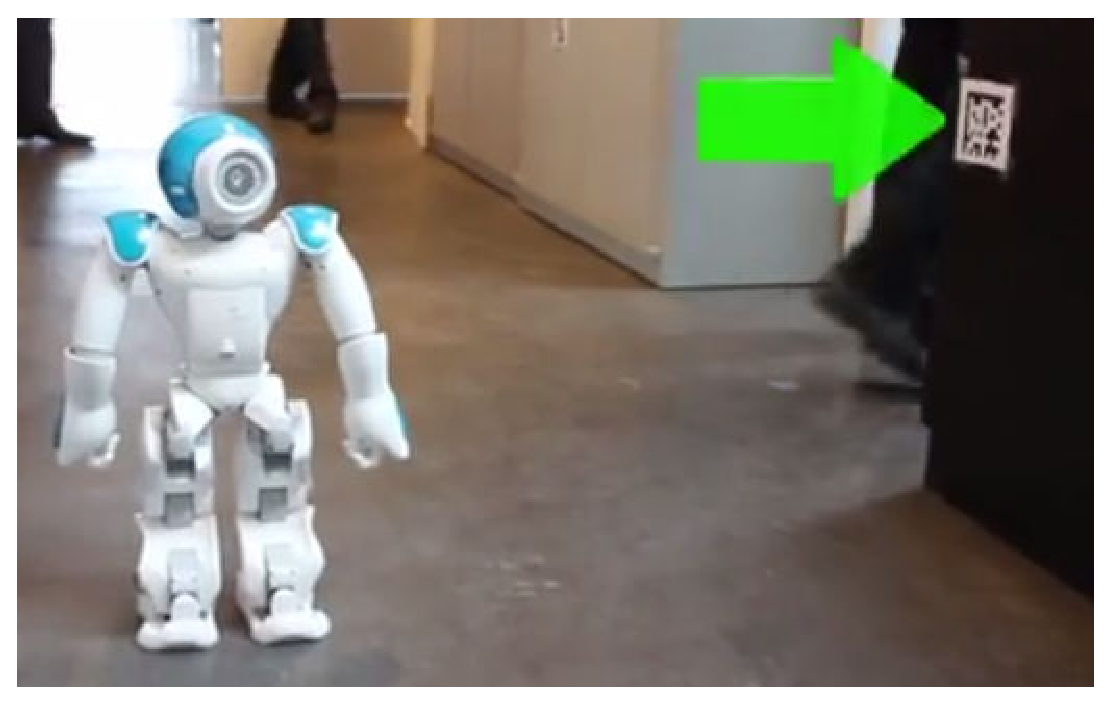
\includegraphics[width=0.5\textwidth]{images/cap2/LocalizacionMarcas.eps}
    \caption{Localización a través de código QR}
    \label{fig:LocalizacionMarcas}
  \end{center}
\end{figure}

Cuando este tipo de marcas no se pueden separar de las imágenes, porque bien no
se tienen puntos de referencia artificiales, o no se puede reconocer del propio
entorno marcas artificiales, se recurre a la localización basada en el análisis
de las imágenes capturadas. El primer paso es el 'autro-aprendizaje',
habitualmente navegar de forma autónoma y recoger las imágenes del entorno.
Estas imágenes se procesan, comparando los elementos en la escena de cada nueva
imagen recogida con la anterior y las imágenes que se tiene en el histórico,
obteniendo así la localización actual.

\begin{figure}[!th]
  \begin{center}
    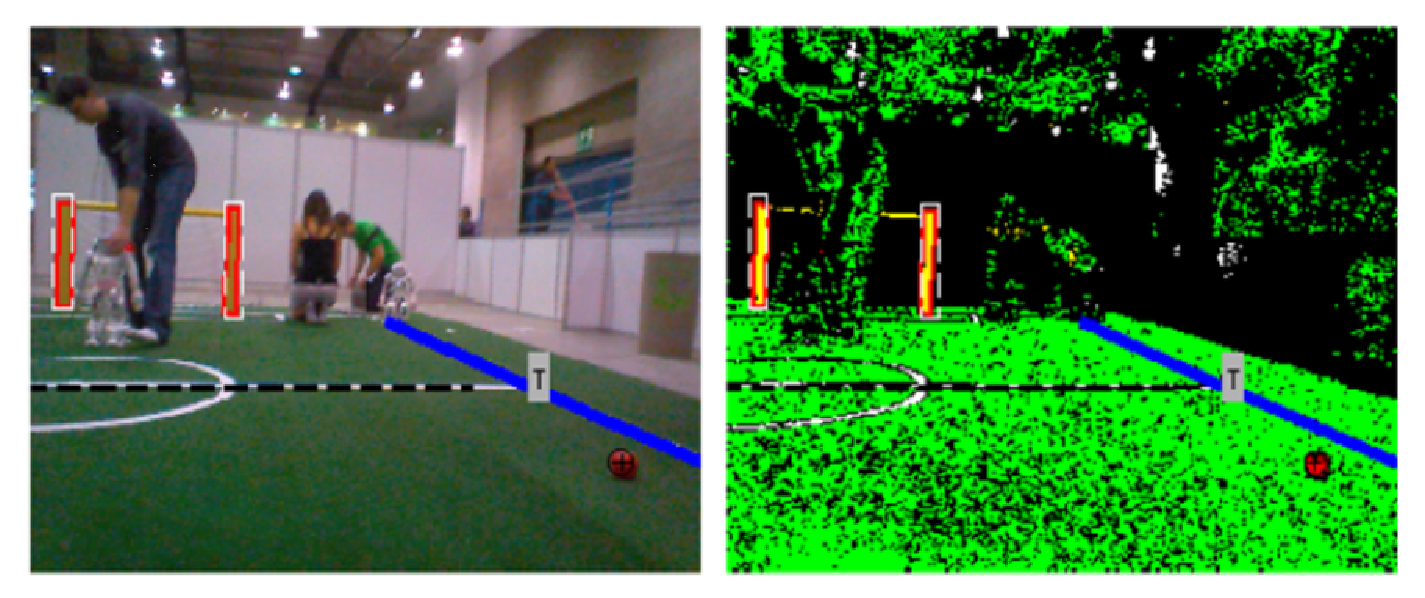
\includegraphics[width=0.5\textwidth]{images/cap2/LocalizacionImagenes.eps}
    \caption{Localización mediante los elementos de la escena}
    \label{fig:LocalizacionImagenes}
  \end{center}
\end{figure}

%--------------------------------------
\subsection{Búsqueda de caminos}
% https://en.wikipedia.org/wiki/Motion_planning
% http://correll.cs.colorado.edu/?p=965
% http://ais.informatik.uni-freiburg.de/teaching/ss11/robotics/slides/18-robot-motion-planning.pdf
% http://rabida.uhu.es/dspace/bitstream/handle/10272/5501/Nuevas_aportaciones_en_algoritmos_de_planificacion.pdf?sequence=2
La búsqueda de caminos permite hallar el conjunto de movimientos que permite a
un robot encontrar el camino más óptico hasta llegar a su objetivo, para no
solamente llegar en el menor tiempo posible, sino también evitar por el camino
los obstáculos que hagan peligrar el estado del robot o simplemente le retrasen.

El problema de la búsqueda de caminos ha sido ampliamente estudiado, existiendo
múltiples algoritmos para solventar este problema. 

Entre los métodos más conocidos están los 'roadmap', los cuales se basan en
construir una descripción de todo el espacio libre en el plano mediante un
grafo. Posteriormente los nodos del grafo se van conectando a partir de las
distancias más cortas entre sí, formando todos los caminos posibles, entre los
que se encuentra el más óptimo.

\begin{figure}[!th]
  \begin{center}
    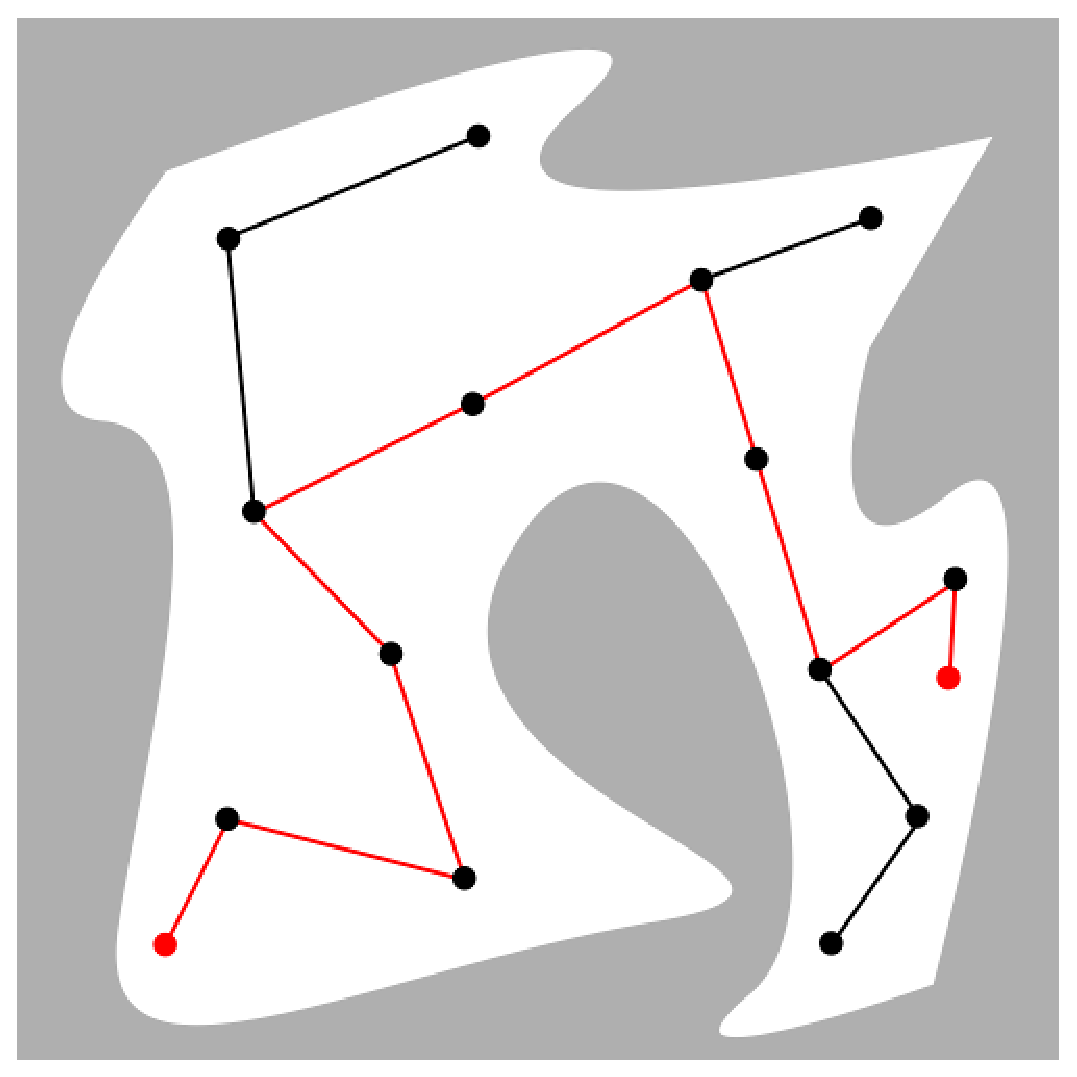
\includegraphics[width=0.5\textwidth]{images/cap2/BusquedaCaminosRoadmap.eps}
    \caption{Ejemplo de un 'roadmap'}
    \label{fig:BusquedaCaminosRoadmap}
  \end{center}
\end{figure}

Por otra parte, existen los métodos de descomposición en celdas, que en vez de
representar el entorno en un grafo, dividen el espacio libre de colisiones en un
conjunto de celdas. 

En los ultimos años han surgido métodos alternativos que permiten dar solución a
la complejidad del entornos y las restricciones cinemáticas que puede presentar
un robot en la búsqueda de caminos, son los algoritmos de generación aleatoria,
el más famoso es el RRT o 'Rapidly Exploring Random Trees', muy utilizados en la
navegación autónoma. Este algoritmo se basa en la construcción al azar de un 
árbol que va creciendode manera incremental mediante la captura de nuevas
muestras del entorno.

%--------------------------------------
\subsection{Mapeo robótico}
% https://en.wikipedia.org/wiki/Robotic_mapping
% https://en.wikipedia.org/wiki/3D_reconstruction_from_multiple_images
% Introduccion sobre el mapeo en robotica, que es porque...

El mapeo robótico 

%--------------------------------------
% \subsection{SLAM} dentro de mapeo...


%++++++++++++++++++++++++++++++++++++++++++++++++++++++++++++++++++++++++++++++


%++++++++++++++++++++++++++++++++++++++++++++++++++++++++++++++++++++++++++++++
